\section{Convex sets}
\subsection{Definitions}
\begin{definition}[Convex set]
    A set $C$ is a \emph{convex set} if every segment that connects two points in $C$ is in $C$. Formally:
    \begin{equation*}
        \forall x, y \in C, \forall \theta \in [0, 1], \quad \theta x + (1 - \theta) y \in C
    \end{equation*}
\end{definition}

\begin{example}
    Here are some examples of convex and non-convex sets:
    \begin{figure}[H]
        \centering
        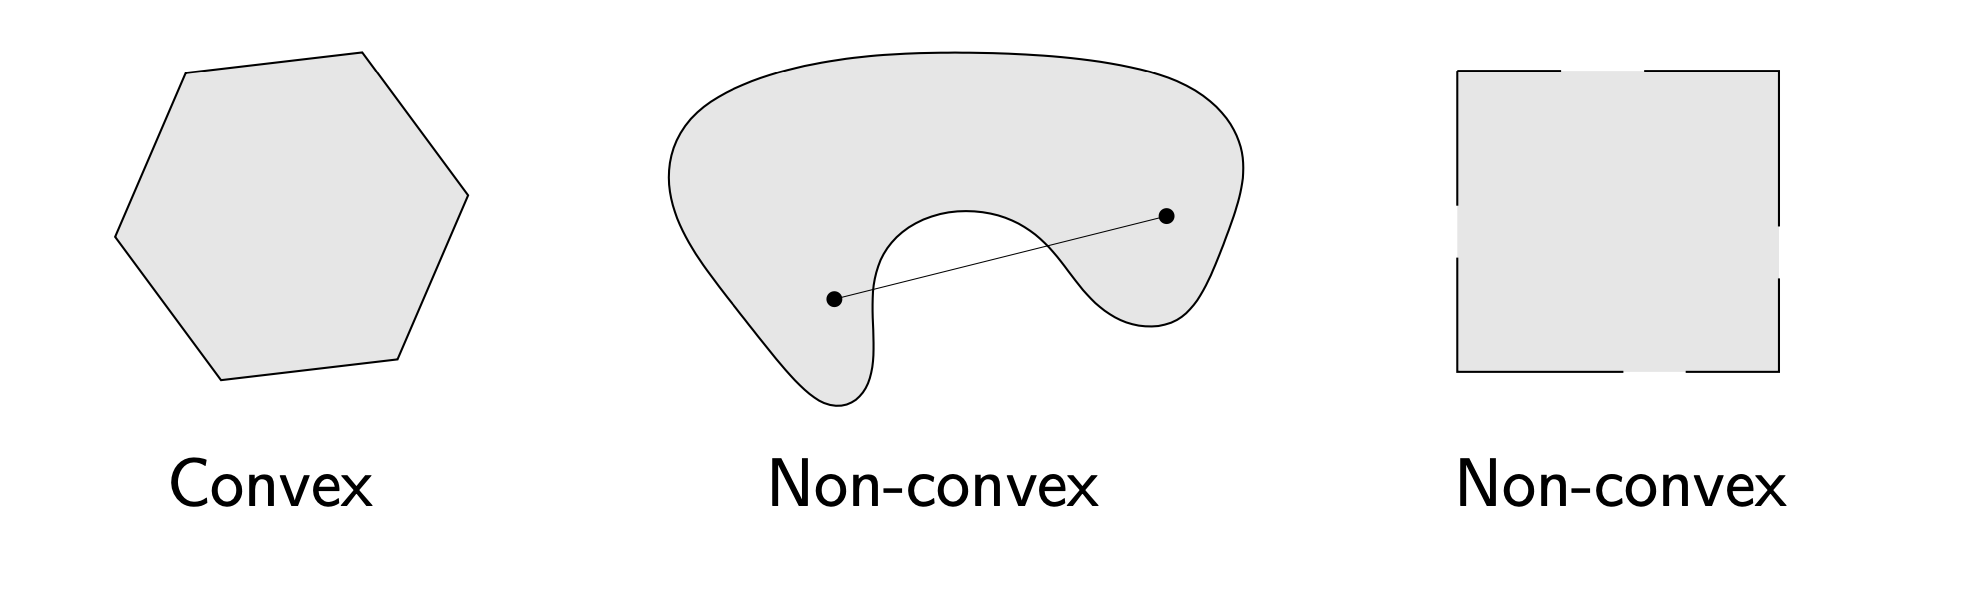
\includegraphics[width=.8\textwidth]{convex-sets/examples.png}
    \end{figure}
\end{example}
In many cases, we will use proper (i.e. non-empty) convex sets, and closed convex sets.

\begin{definition}[Convex hull]
    The \emph{convex hull} of $S$, denoted $\Conv(S)$, is the smallest convex set that contains $S$.
\end{definition}

\begin{definition}[Convex combinations]
    The \emph{convex combinations} of $x_1, \dots, x_k$ are all the point $x$ of the form:
    \begin{equation*}
        x = \theta_1x_1 + \dots + \theta_kx_k
    \end{equation*}
    with $\theta_1, \dots, \theta_k \geq 0$ and $\sum_{i=1}^k\theta_i = 1$.
\end{definition}

\begin{property}
    The convex hull of a set $S$ is the set of all convex combinations of points in $S$:
    \begin{equation*}
        \Conv(S) = \set{\sum_{i=1}^k\theta_ix_i}{(x_i)\in S^k, (\theta_i)\in\R_+^k, \sum_{i=1}^k\theta_i = 1}
    \end{equation*}
\end{property}

\subsection{Examples}
\subsubsection{Hyperplanes and halfspaces}
\begin{definition}[Hyperplane]
    A \emph{hyperplane} is the set of the form:
    \begin{equation*}
        H = \set{x}{a^\tp x = b}
    \end{equation*}
    for some $a\in\R^n\setminus\{0\}$ and $b\in\R$. $a$ is called the \emph{normal vector} of $H$. Hyperspaces are affine and convex.

    \begin{figure}[H]
        \centering
        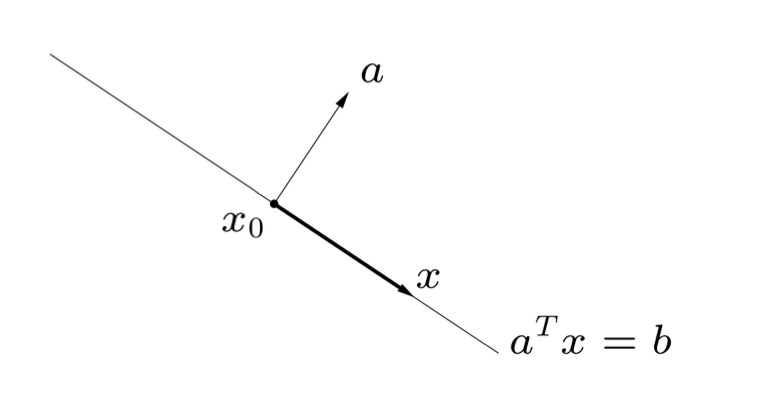
\includegraphics[width=.5\textwidth]{convex-sets/hyperplane.png}
        \caption{Hyperplane}
    \end{figure}
\end{definition}

\begin{definition}[Halfspace]
    A \emph{halfspace} is the set of the form:
    \begin{equation*}
        H = \set{x}{a^\tp x\leq b}
    \end{equation*}
    for some $a\in\R^n\setminus\{0\}$ and $b\in\R$. $a$ is called the \emph{normal vector} of $H$. Halfspaces are convex.

    \begin{figure}[H]
        \centering
        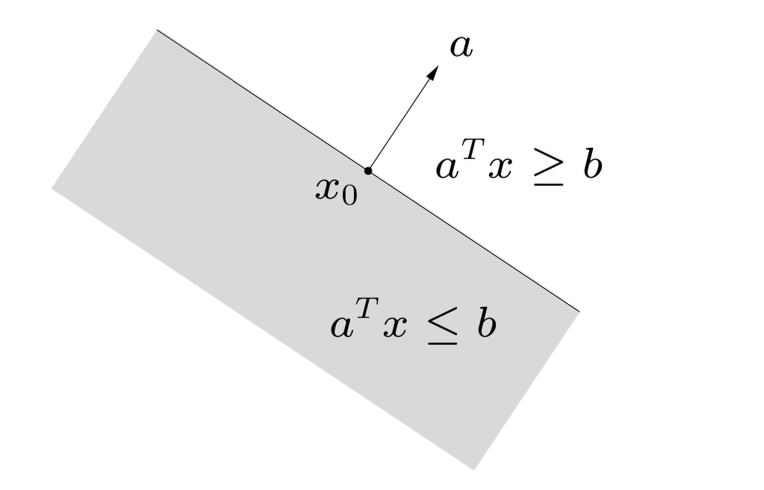
\includegraphics[width=.5\textwidth]{convex-sets/halfspace.png}
        \caption{Halfspace}
    \end{figure}
\end{definition}

\subsubsection{Euclidian balls and ellipsoids}
\begin{definition}[Euclidian ball]
    The \emph{Euclidian ball} of center $x_c$ and radius $r$ is the set:
    \begin{equation*}
        B(x_c, r) = \set{x}{\norm{x - x_c}_2\leq r} = \set{x_c+ru}{\norm{u}_2\leq 1}
    \end{equation*}
    Euclidian balls are convex.
\end{definition}

\begin{definition}[Ellipsoid]
    An \emph{ellipsoid} is the set of the form:
    \begin{equation*}
        E = \set{x}{(x - x_c)^\tp P^{-1}(x - x_c)\leq 1}
    \end{equation*}
    with $P\in\Sb^n_{++}$\footnote{$\Sb^n_{++}$ denotes the set of symmetric positive definite matrices of size $n$} and $x_c\in\R^n$. Ellipsoids are convex.

    \begin{figure}[H]
        \centering
        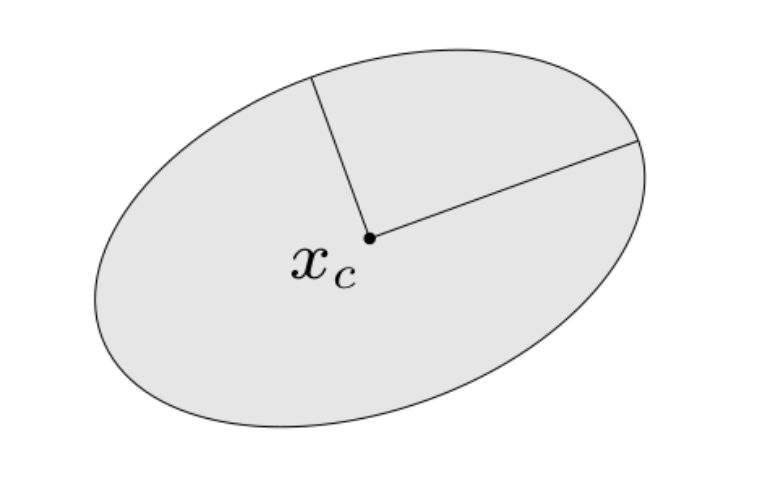
\includegraphics[width=.3\textwidth]{convex-sets/ellipsoid.png}
        \caption{Ellipsoid}
    \end{figure}

    An alternative representation of an ellipsoid is:
    \begin{equation*}
        E = \set{x_c + Au}{\norm{u}_2\leq 1}
    \end{equation*}
    for some nonsingular matrix $A\in\textnormal{GL}_n(\R)$. We can choose $A$ symmatric and positive definite without loss of generality, for instance by choosing $A = P^{1/2}$.
\end{definition}

\subsubsection{Cones}
\begin{definition}[Cones]
    A set $K$ is a \emph{cone}, or a \emph{nonnegative homogeneous set}, if:
    \begin{equation*}
        \forall x\in K, \forall \theta\in\R_+^*, \quad \theta x\in K
    \end{equation*}

    \begin{figure}[H]
        \centering
        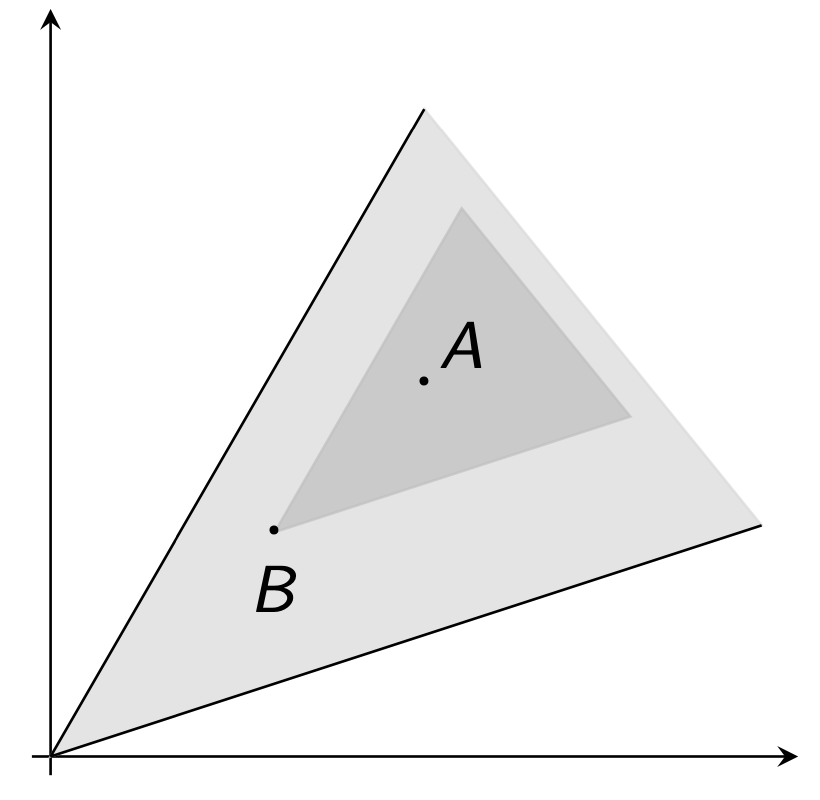
\includegraphics[width=.6\textwidth]{convex-sets/cone.png}
    \end{figure}
\end{definition}

\begin{definition}[Convex cone]
    A set $K$ is a \emph{convex cone} if:
    \begin{equation*}
        \forall x_1, x_2\in K, \forall \theta_1, \theta_2\in\R_+^*, \quad \theta_1x_1 + \theta_2x_2\in K
    \end{equation*}

    \begin{figure}[H]
        \centering
        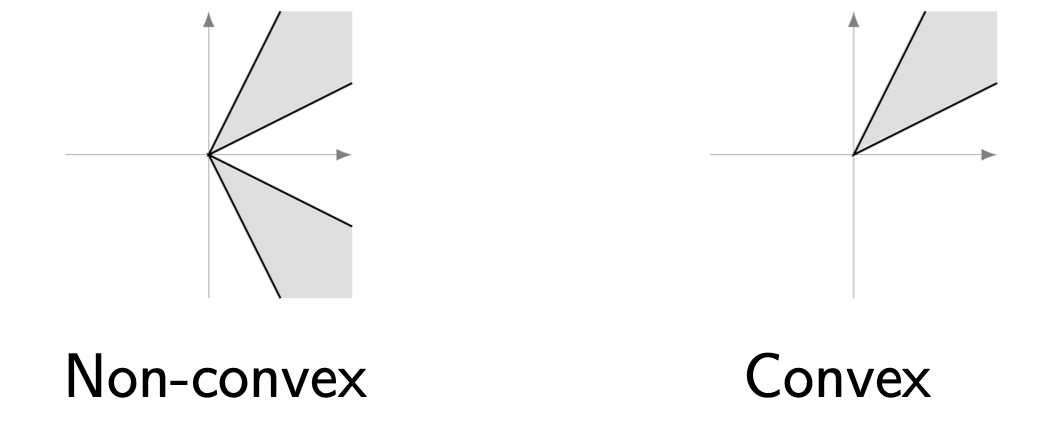
\includegraphics[width=.45\textwidth]{convex-sets/convex-cones.png}
    \end{figure}
\end{definition}

In the followings, we will denote by:
\begin{itemize}
    \item $\Sb^n\subset\R^{n\times n}$ the set of symmetric matrices of size $n$
    \item $\Sb^n_+$ the set of positive semidefinite matrices of size $n$, that is matrices verifying:
    \begin{equation*}
        \forall z\in\R^n, z^\tp Xz\geq 0
    \end{equation*}
    also denoted $X\succcurlyeq 0$.
    \item $\Sb^n_{++}$ the set of positive definite matrices of size $n$, that is matrices verifying:
    \begin{equation*}
        \forall z\in\R^n, z^\tp Xz > 0
    \end{equation*}
    also denoted $X\succ 0$.
\end{itemize}
$\Sb^n_+$ and $\Sb^n_{++}$ are convex cones.

Special cases of cones include:
\begin{description}
    \item[Positive orthant] $K = \R_+^n = \set{x\in\R^n}{x_i\geq 0, \forall i}$
    \item[Norm cones] $K = \set{(x, t)\in\R^n\times\R}{\norm{x}\leq t}$. A particular case is the second-order cone (SOC), based on the $\ell_2$ norm.
    \begin{figure}[H]
        \centering
        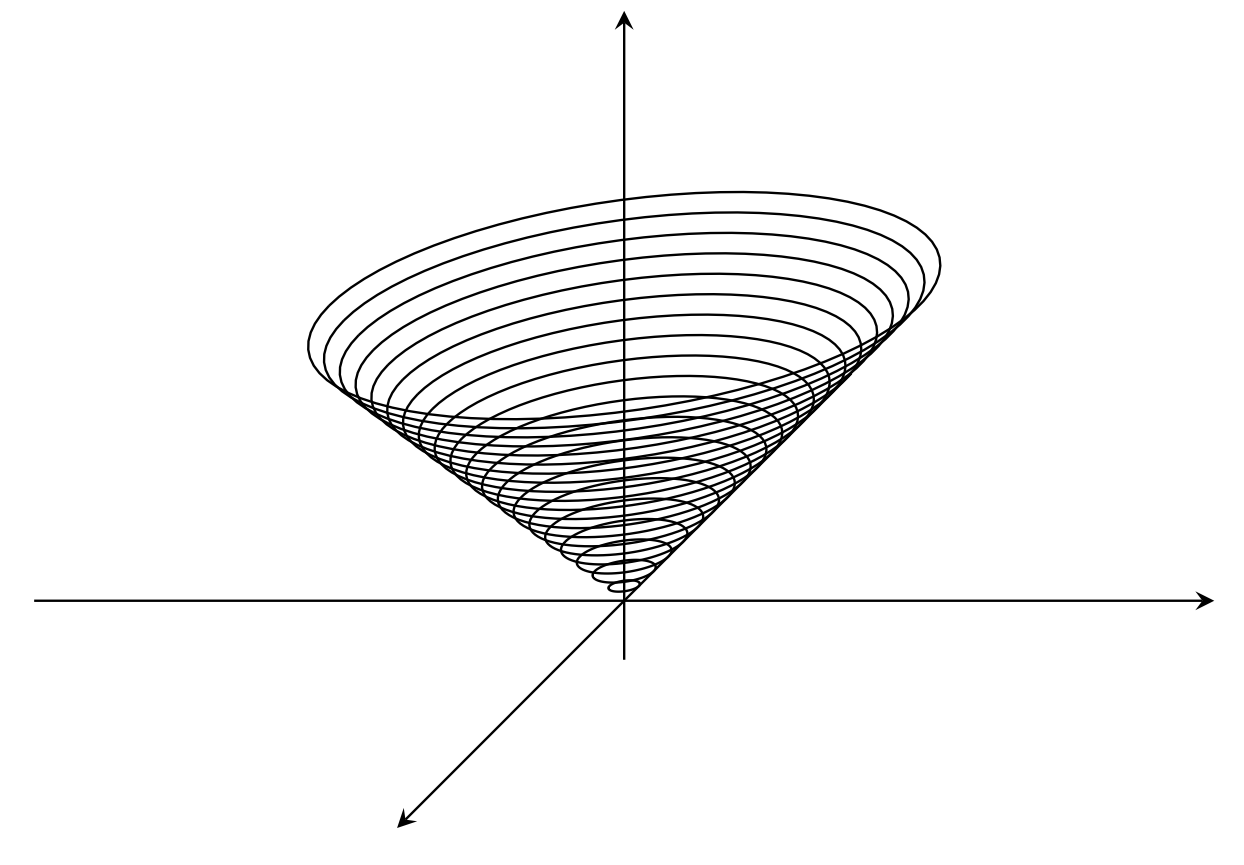
\includegraphics[width=.4\textwidth]{convex-sets/soc.png}
    \end{figure}
    \item[Positive polynomials] $K_n = \set{x\in\R^{n+1}}{\forall t\in\R, \sum_{i=0}^n x_i t^i \geq 0}$
    \item[Positive semidefinite cone] $\Sb^n_+ = \set{X\in\Sb^n}{\forall z\in\R^n, z^\tp Xz\geq0}$ 
    \item[Co-positive cone] $\Sb^n_+ = \set{X\in\Sb^n}{\forall z\in\R^n_+, z^\tp Xz\geq0}$ 
    \item[Exponential cone] $\set{(x,y,z)\in\R\times\R_+^*\times\R}{z\geq ye^{x/y}}$ 
\end{description}

\begin{definition}[Dual cones]
    The \emph{dual cone} to a convex cone $K$ is the set:
    \begin{equation*}
        K^* = \set{y}{\forall x\in K,\quad y^\tp x\geq 0}
    \end{equation*}
    Convex cones and their duals are particularly useful for convex duality. A convex cone that satisfies $K=K^*$ is called \emph{self-dual}.
\end{definition}

\begin{definition}[Polar cones]
    The \emph{polar cone} to a convex cone $K$ is the set:
    \begin{equation*}
        K^\diamond = \set{y}{\forall x\in K,\quad y^\tp x\leq 0}
    \end{equation*}
    We have the identity $K^\diamond = -K^*$.
\end{definition}

\subsection{Convexity-preserving operations}
To establish the convexity of a set $C$, the most basic approach is to apply the definition by proving that every segment that connects two points in $C$ is in $C$. However, this can be tedious in practice. Instead, we can use operations that preserve convexity.

\subsubsection{Intersection and union}
\begin{property}[Convexity is preserved by intersection]
    For any convex sets $C_1$ and $C_2$, the intersection $C_1\cap C_2$ is convex.
\end{property}
Likewise, the intersection of an arbitrary number of convex sets is convex.

\begin{figure}[H]
    \centering
    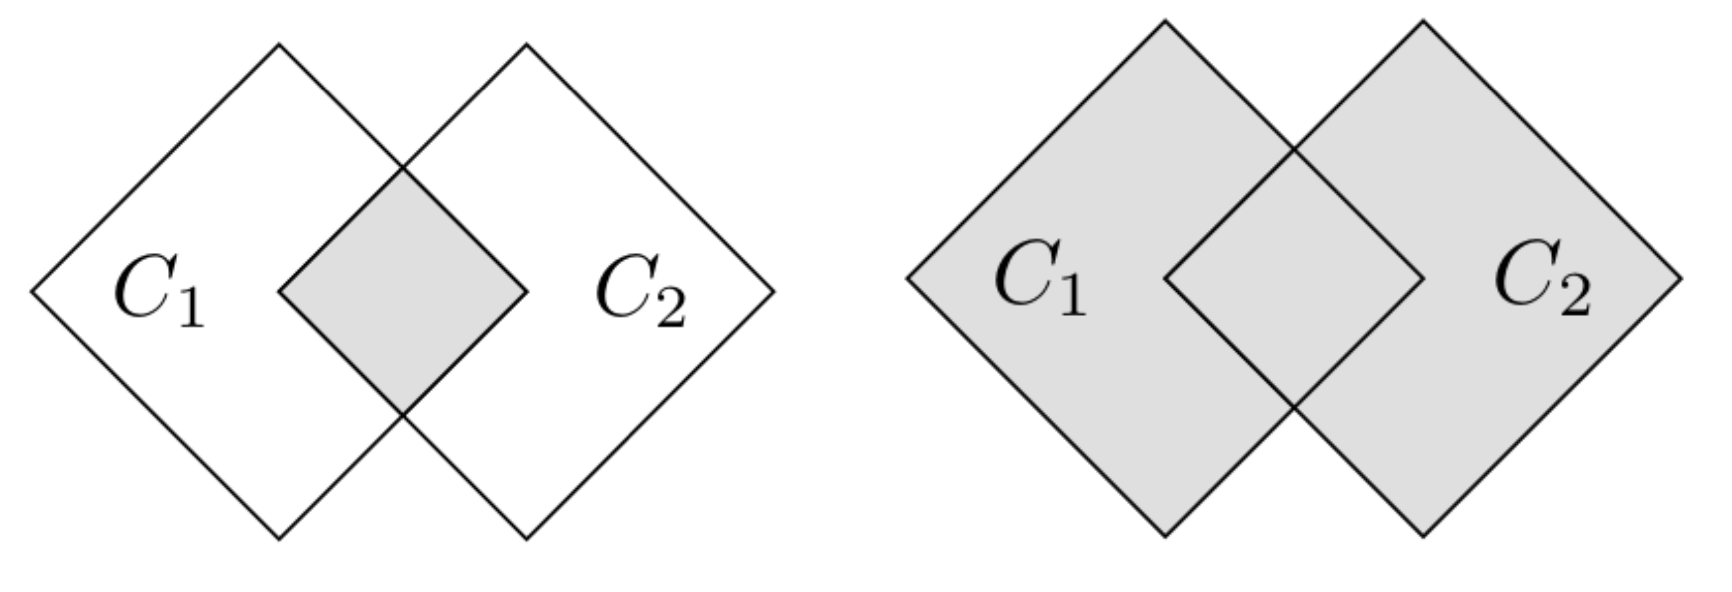
\includegraphics[width=.6\textwidth]{convex-sets/union-intersection.png}
\end{figure}

\begin{remark}
    The union of convex sets is not necessarily convex. For instance in $\R$, both $[0, 1]$ and $[2, 3]$ are convex, but their union $[0, 1]\cup[2, 3]$ is not.
\end{remark}

\begin{definition}[Polyhedron]
    A \emph{polyhedron} is the solution set of finitely many linear inequalities and equalities:
    \begin{equation*}
        S = \set{x\in\R^n}{Ax\leq b, Cx=d}
    \end{equation*}
    for $A\in\mathscr{M}_{m,n}(\R)$ and $C\in\mathscr{M}_{p,n}(\R)$. Polyhedra are convex, since they are the intersection of halfspaces and hyperplanes which are convex.
\end{definition}
\begin{figure}[H]
    \centering
    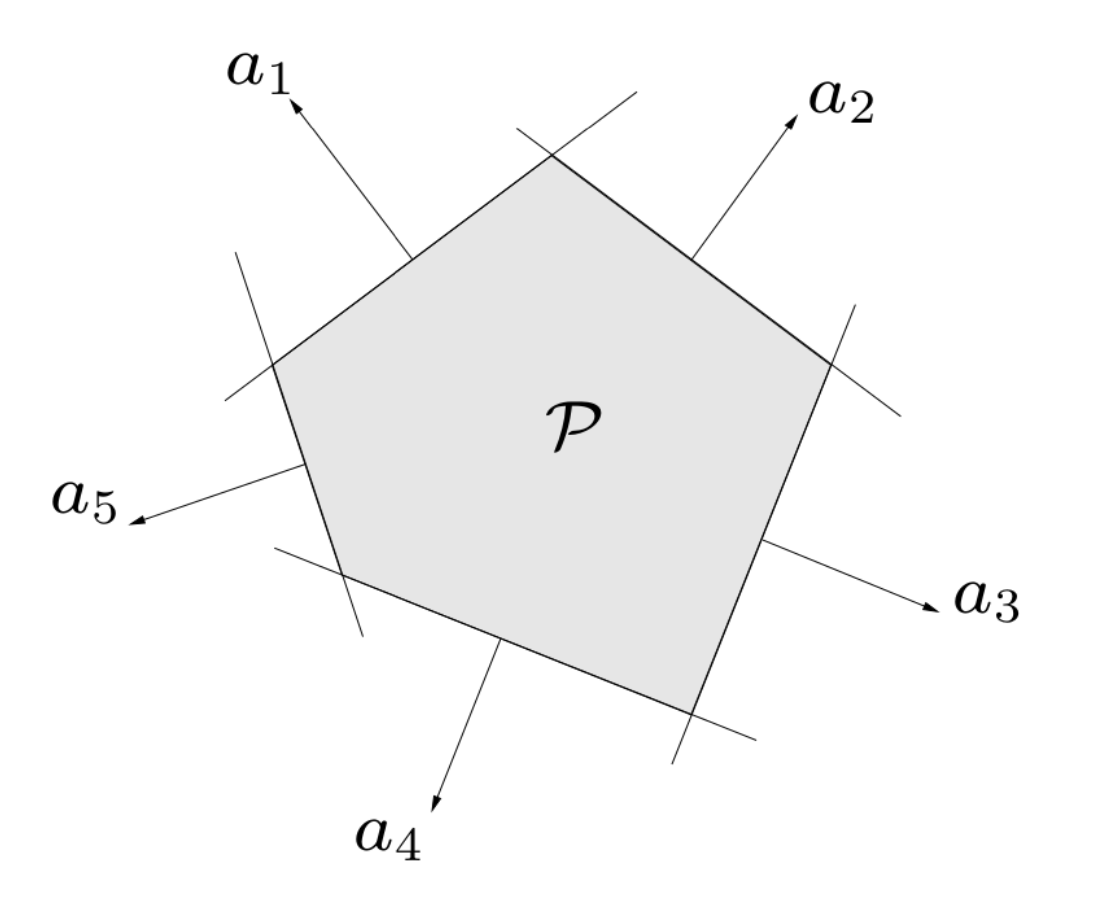
\includegraphics[width=.4\textwidth]{convex-sets/polyhedron.png}
\end{figure}

\begin{example}
    Let:
    \begin{equation*}
        S = \set{x\in\R^m}{\forall t\in\R, \quad |t|\leq\frac{\pi}{3} \implies \left|\sum_{k=1}^m x_k\cos(kt)\right|\leq 1}
    \end{equation*}
    $S$ is convex, since it can be written as the intersection of convex sets.
    \begin{figure}[H]
        \centering
        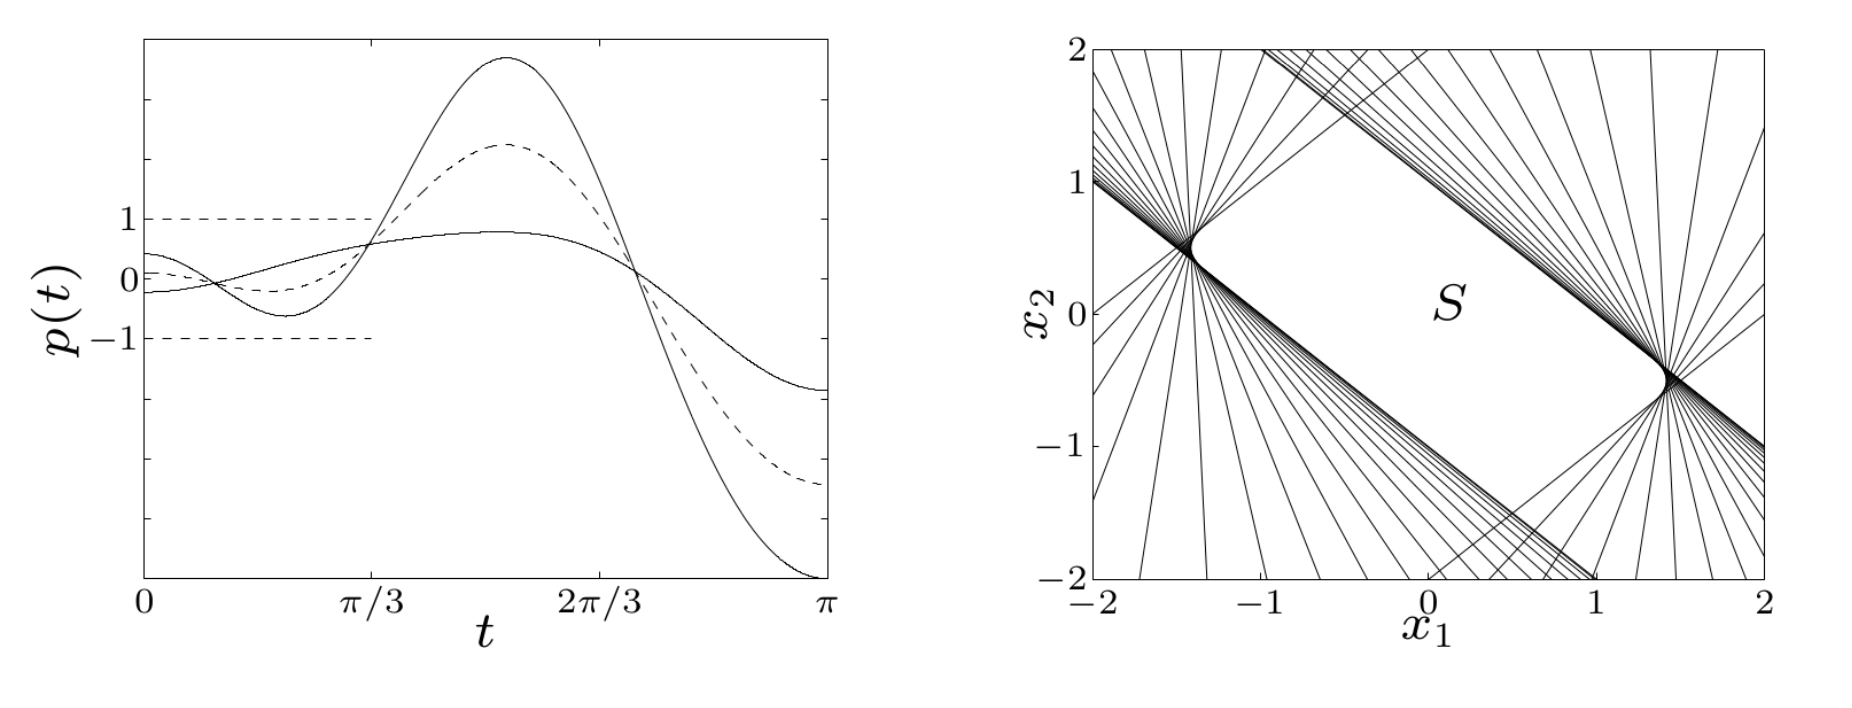
\includegraphics[width=.7\textwidth]{convex-sets/examples-cos.png}
    \end{figure}
\end{example}

\begin{example}
    $\Sb^n_+$ is convex since it is the intersection of convex sets:
    \begin{equation*}
        \Sb^n_+ = \set{X\in\Sb^n}{\forall z\in\R^n, z^\tp Xz\geq 0} = \Sb^n \cap \bigcap_{z\in\R^n} \set{X\in\mathscr{M}_n(\R)}{z^\tp Xz\geq 0}
    \end{equation*}
    Each set $\set{X\in\mathscr{M}_n(\R)}{z^\tp Xz\geq 0}$ being convex, their intersection is convex. In particular, it doesn't matter if the number of sets is finite, countable or uncountable.
\end{example}

\subsubsection{Affine functions}
\begin{property}[The image of a convex set by an affine function is convex]
    If $L:\R^n\to\R^m$ is an affine function, then if $C$ is convex, $L(C)$ is convex.
\end{property}

More explicitly, let $A\in\mathscr{M}_{m,n}(\R)$ and $b\in\R^m$. The affine function $L(x) = Ax + b$ maps $C$ to $L(C) = \set{y\in\R^m}{\exists x\in C, y = Ax + b}$, which is convex if $C$ is convex.

\begin{property}[The pre-image of a convex set by an affine function is convex]
    If $L:\R^n\to\R^m$ is an affine function, then $L^{-1}(C)$, the pre-image of $C$ by $L$ defined by:
    \begin{equation*}
        L^{-1}(C) = \set{x\in\R^n}{L(x)\in C}
    \end{equation*}
    is convex if $C$ is convex.
\end{property}

\begin{example}[Linear matrix inequalities]
    Let $A_1, \dots, A_m\in\Sb^n(\R)$. The set:
    \begin{equation*}
        \set{x\in\R^m}{\sum_{i=1}^m x_iA_i\succcurlyeq 0}
    \end{equation*}
    is an affine pre-image of $\Sb_+^n$ for the mapping $L:\R^m\to\Sb^n$ defined by:
    \begin{equation*}
        L(x) = \sum_{i=1}^m x_iA_i
    \end{equation*}
    $\Sb_+^n$ being convex, the set is convex. $\sum_{i=1}^m x_iA_i\succcurlyeq 0$ is called a \emph{linear matrix inequality}.
\end{example}

\subsection{Geometric elements}
\subsubsection{Separating and supporting hyperplanes}
\begin{property}[Separating hyperplanes]
    Soppose that $C, D\subseteq\R^n$ are two non-intersecting convex sets (that is $C\cap D = \emptyset$). Then there exists a hyperplane that separates $C$ and $D$, that is:
    \begin{equation*}
        \exists s\in\R^n\setminus\{0\}, \exists r\in\R, \quad \forall x\in C, s^\tp x\leq r \quad \text{and} \quad \forall x\in D, s^\tp x\geq r
    \end{equation*}
    where $\set{x\in\R^n}{s^\tp x = t}$ is called the \emph{separating hyperplane}.
    \begin{figure}[H]
        \centering
        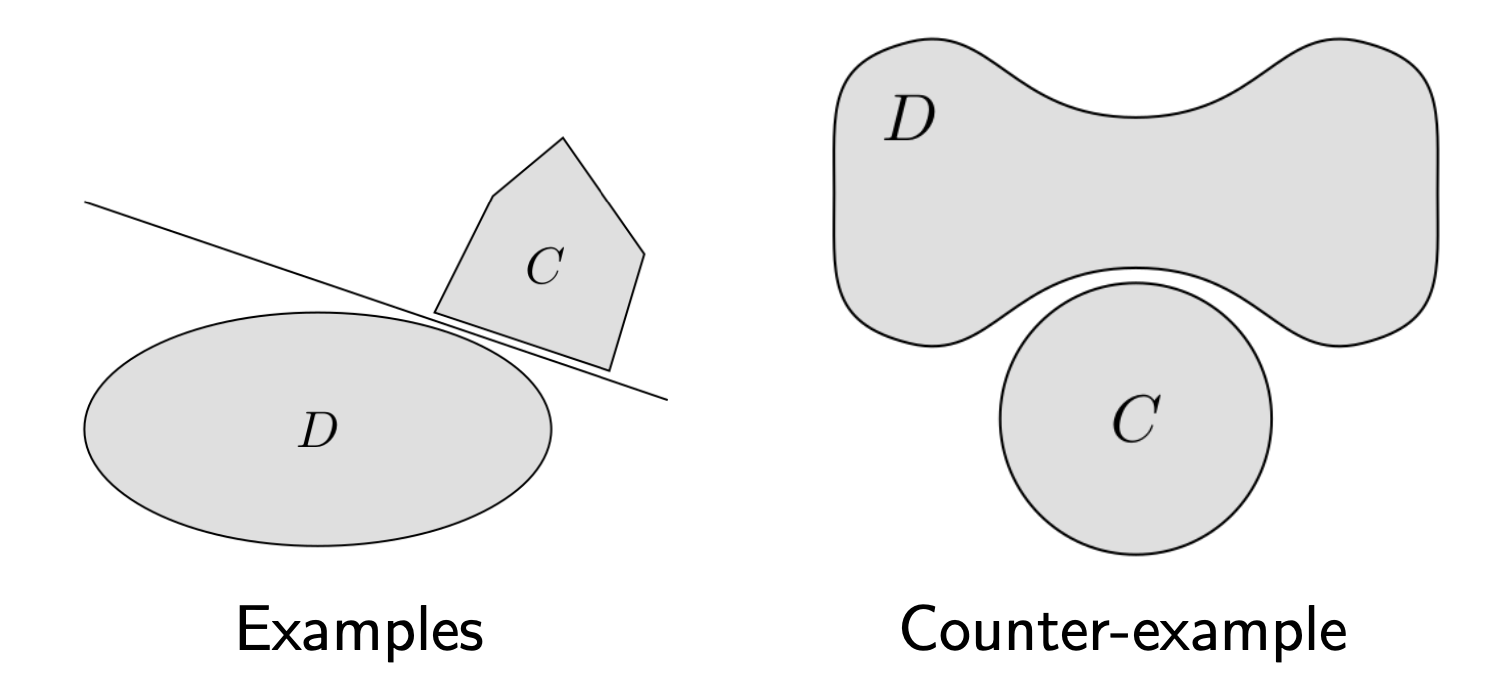
\includegraphics[width=.6\textwidth]{convex-sets/separating-hyperplane.png}
    \end{figure}
\end{property}

\begin{property}[Strict separating hyperplanes]
    Suppose that $C, D\subseteq\R^n$ are two non-intersecting \textbf{closed} convex sets, and that one of them is compact (closed and bounded in finite dimension). Then there exists a hyperplane that strictly separates $C$ and $D$, that is:
    \begin{equation*}
        \exists s\in\R^n\setminus\{0\}, \exists r\in\R, \quad \forall x\in C, s^\tp x< r \quad \text{and} \quad \forall x\in D, s^\tp x> r
    \end{equation*}
    \begin{figure}[H]
        \centering
        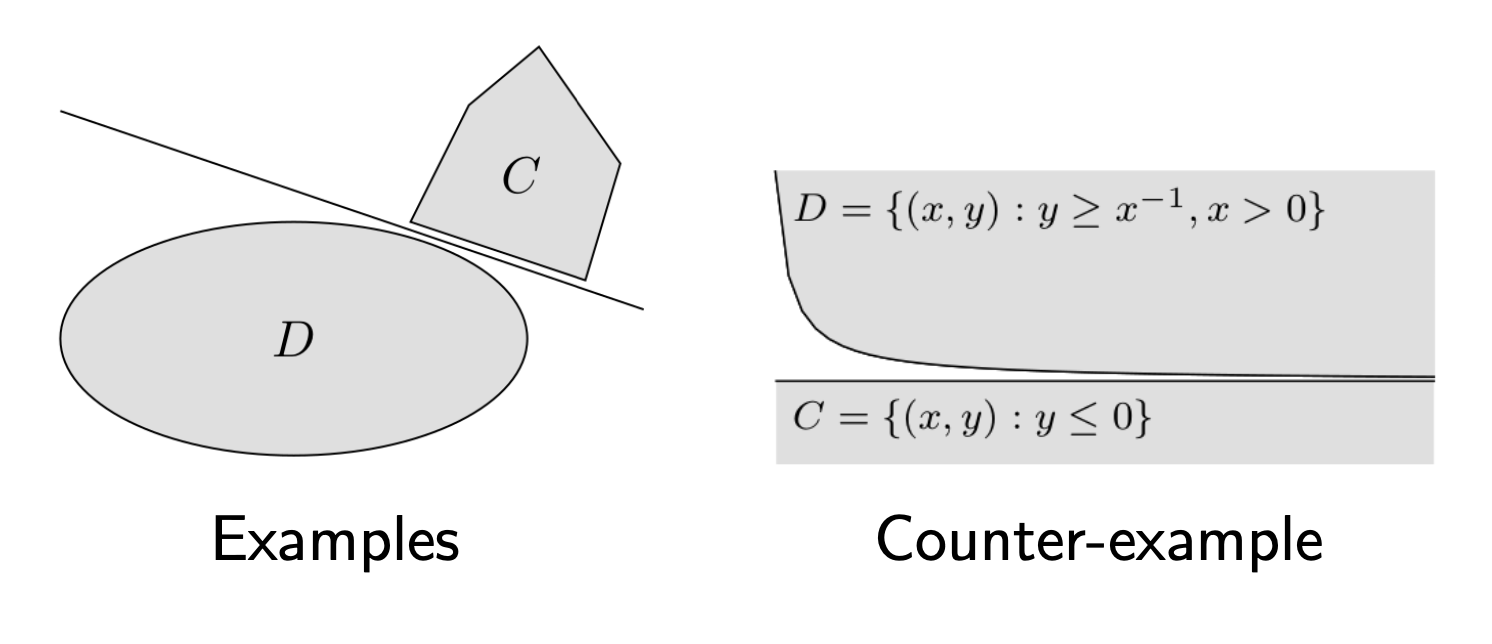
\includegraphics[width=.6\textwidth]{convex-sets/strict-separation.png}
    \end{figure}
\end{property}

Note that a closed convex set $C$ is the intersection of all halfspaces that contain it.
\begin{figure}[H]
    \centering
    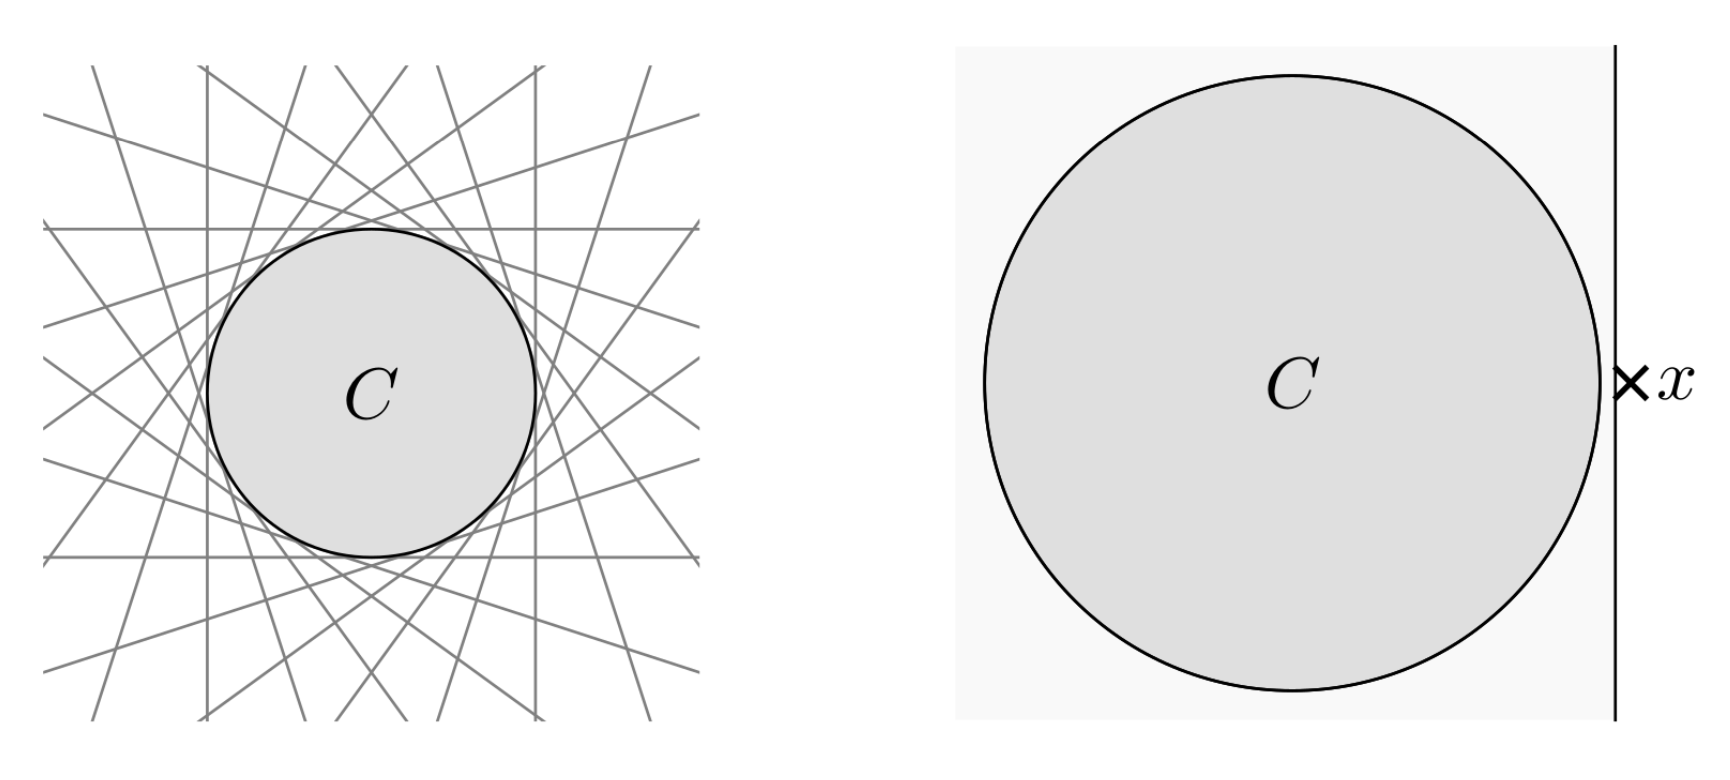
\includegraphics[width=.6\textwidth]{convex-sets/closed-intersection.png}
\end{figure}

\begin{definition}[Supporting hyperplanes]
    Supporting hyperplanes touch the boundary of a convex set, and have the entire set on one side. Formally, a hyperplane $H = \set{y}{s^\tp y=r}$ is a \emph{supporting hyperplane} to a convex set $C$ at a point $x\in\partial C$ if:
    \begin{equation*}
        x^\tp x = r \qquad \text{and} \qquad \forall y\in C, \quad a^\tp y\leq r = s^\tp x
    \end{equation*}
    We also say that $H$ \emph{supports} $C$ at $x$.
    \begin{figure}[H]
        \centering
        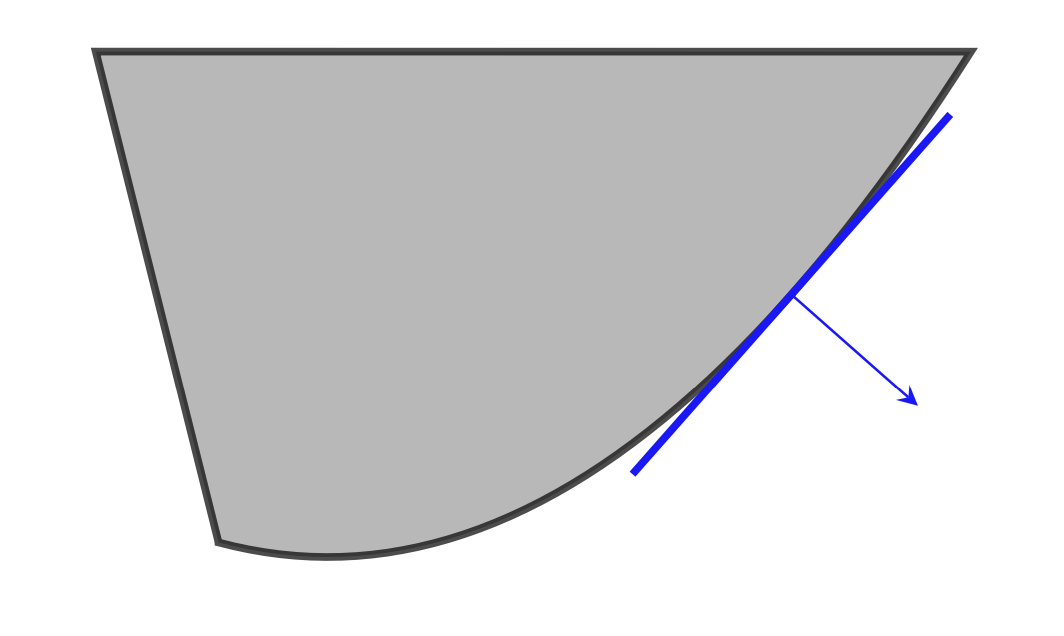
\includegraphics[width=.4\textwidth]{convex-sets/supporting-hyperplane.png}
    \end{figure}
\end{definition}

\begin{property}
    Let $C\subseteq\R^n$ be a non-empty convex set, and let $x\in\partial C$. Then there exists a supporting hyperplane to $C$ at $x$.
\end{property}

\subsubsection{Cone operators}
\begin{definition}[Normal cone operator]
    The \emph{normal cone operator} to a set $C$ at a point $x$ is the set:
    \begin{equation*}
        N_C(x) = \begin{cases*}
            \set{g\in\R^n}{\forall y\in C, \quad g^\tp(y - x)\leq 0} & if $x\in C$\\
            \emptyset & if $x\notin C$
        \end{cases*}
    \end{equation*}
    Intuitively, it is the set of vectors $g$ that form obtuse angles for all $y-x$ with $y\in C$.
\end{definition}

For $x\in \mathring{C}$, we have $N_c(x)=\{0\}$. For $x\in\partial C$, $N_C(x)$ is the set of the normal vectors to the supporting hyperplanes to $C$ at $x$. If $x\notin C$, $N_C(x)$ is empty.

\begin{definition}[Tangent vector]
    Let $C\subseteq\R^n$ be a convex set. A vector $d\in\R^n$ is tangent to $C$ at $x$ if:
    \begin{equation*}
        \exists \{x_k\}_k\subseteq C, \exists \{\lambda_k\}_k\subset\R_+, \quad \lim_{k\to+\infty} \lambda_k (x_k-x) = d
    \end{equation*}
    \begin{figure}[H]
        \centering
        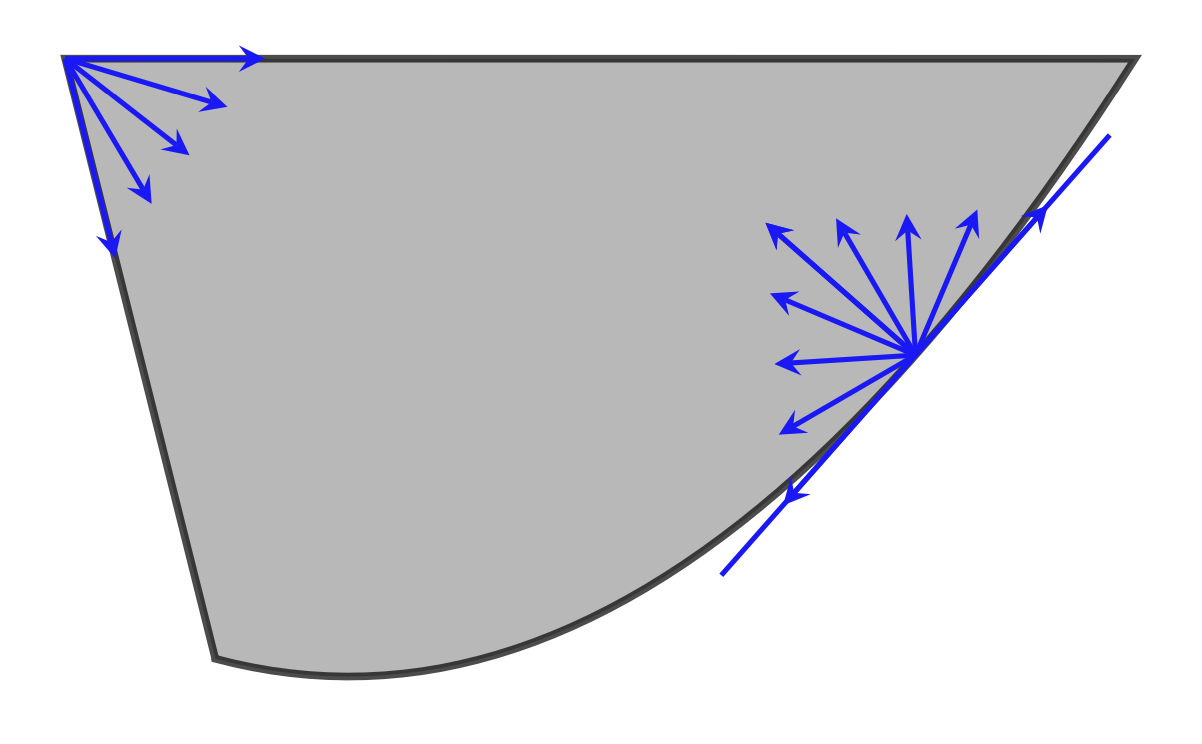
\includegraphics[width=.4\textwidth]{convex-sets/tangent-cone.png}
    \end{figure}
\end{definition}

\begin{definition}[Tangent cone]
    The tangent cone of a convex set $C$ at $x$ is:
    \begin{equation*}
        T_C(x) = N_C^\diamond(x)
    \end{equation*}
\end{definition}